\documentclass[12pt]{article}
\usepackage[utf8]{inputenc}
\usepackage{amsmath}
\usepackage{graphicx}
\usepackage{float}
\usepackage[margin=1in]{geometry}
\usepackage{lineno}
\setlength{\parindent}{2em}
\setlength{\parskip}{1em}
\renewcommand{\baselinestretch}{1.2}
\newcommand\dbyd[2]{\frac{\mathrm d{#1}}{\mathrm d{#2}}}
\newcommand{\R}{\mathcal{R}}
\title{Intensional infect proportion of newborn, with disease induced mortality rate}

\begin{document}
\linenumbers
\maketitle

\section{Motivation}

Previous analysis showed no obvious advantage for intentional infection. But those are the cases where we ignored disease induced mortality. In reality, if we are taking smallpox for example, past researches have determined the mortality rate to be 30 percent for normally infected cases, but only 1 percent for variolated cases. Thus, it is possible that intentional infection has a positive effect on disease control.

\section{Introduction}

Again, we consider two intentional infect strategies. One is to intentional infect newborns and the other is to intentional infect susceptible. In this document, we discuss the first strategy only.

\section{System of differential equations}
Since we have to consider disease induced mortality rate, we need to adjust our model by adding extra terms representing mortality rate.

The following assumptions are used:

\begin{itemize}
\item Birth and natural death rate are the same.
\item The latent period is short enough to be ignored.
\item All susceptible individuals are equally likely to be infected, and all infected individuals are equally infectious.
\end{itemize}

\begin{equation}\label{1}
\begin{split}
\dbyd{S}{t}&=\mu(1-p)- \beta S(V+I)-\mu S \,,\\
\dbyd{V}{t}&=\beta SV+\mu p-\gamma V -\mu V\,,\\
\dbyd{I}{t}&=\beta SI-\gamma I -\mu I\,,\\
\dbyd{M}{t}&=0.01\gamma V+0.3\gamma I\,,\\
\dbyd{R}{t}&=0.99\gamma V+0.7\gamma I-\mu R\,,
\end{split}
\end{equation}

Here, $\beta$ is the transmission rate, $\gamma$ is the recovery rate,
$\mu$ is the \emph{per capita} rate of birth and death, $p$ is the
proportion of newborns that are intentionally infected.

For simplicity, we now convert the system into dimensionless form using dimensionless time coordinate,
\begin{equation}
\tau=(\gamma+\mu)t \,,
\end{equation}

As the result, we obtain,

\begin{subequations}\label{1}
\begin{align}
\dbyd{S}{\tau}&=\epsilon(1-p)- \R_0 S(V+I)-\epsilon S\,, \\
\dbyd{V}{\tau}&=\R_0 SV+\epsilon p-V\,,\\
\dbyd{I}{\tau}&=\R_0 SI-I\,,\\
\dbyd{M}{\tau}&=0.01(1-\epsilon) V+0.3(1-\epsilon) I\,,\\
\dbyd{R}{\tau}&=0.99(1-\epsilon) V+0.7(1-\epsilon) I-\epsilon R\,,
\end{align}
\end{subequations}

where $\epsilon=\frac{\mu}{\gamma+\mu}$, $\R_0=\frac{\beta}{\gamma+\mu}$.

\section{Endemic Equilibrium}

To find endemic equilibrium, first we let equation (3c) equal to 0, we get: $I=0$ or $S=\frac{1}{\R_0}$. If $S=\frac{1}{\R_0}$, then by substituting into (3b), we get:
\begin{equation}
\dbyd{V}{\tau}=\epsilon p = 0.
\end{equation}

Since $\epsilon\neq0$, we necessarily have $p=0$, which is again, a trivial case where no intentional infection is involved and we do not consider this case here. Thus, we conclude that $I=0$.

We use this to substitute back into equation (3a) and (3b), and letting all equations equal to zero, we get:

\begin{subequations}
\begin{align}
\hat{S}&= \frac{1}{\R_0}-\frac{2p}{(\R_0 -1)+ \sqrt{(\R_0-1)^2+4\R_0 p}}\,,\\
\hat{V}&= \frac{\epsilon(\R_0 -1)+ \epsilon \sqrt{(\R_0-1)^2+4\R_0 p}}{2\R_0}\,, \\
\hat{I}&=0\,,\\
\end{align}
\end{subequations}

Stability analysis rely on Jacobian Matrix,
\begin{equation}
\mathcal{J} =
\begin{bmatrix}
    \ -\R_0 (V+I)-\epsilon       & -\R_0 S     &-\R_0 S\\
    \ \R_0 V       & \R_0 S-1    &0\\
    \ \R_0 I       &0     &\R_0 S-1\\
\end{bmatrix}\,.
\end{equation}

Eigenvalues of Jacobian are given as follow,
\begin{subequations}
\begin{align}
\lambda_1&=-1+\R_0 S\\
\lambda_2&=\frac{-1-\epsilon+\R_0 S-\R_0 V-i\R_0-\sqrt{(-1-\epsilon+\R_0 S-\R_0 V-i\R_0)^2+4(-\epsilon-i\R_0+\epsilon\R_0 S-\R_0 V)}}{2}\\
\lambda_3&=\frac{-1-\epsilon+\R_0 S-\R_0 V-i\R_0+\sqrt{(-1-\epsilon+\R_0 S-\R_0 V-i\R_0)^2+4(-\epsilon-i\R_0+\epsilon\R_0 S-\R_0 V)}}{2}
\end{align}
\end{subequations}

By using equation (5a), we acquire the following:
\begin{equation}
\hat{S}=\frac{1}{\R_0}-\frac{2p}{(\R_0 -1)+ \sqrt{(\R_0-1)^2+4\R_0 p}}\,,
\end{equation}
Thus,
\begin{equation}
\R_0\hat{S}=1-\frac{2p\R_0}{(\R_0 -1)+ \sqrt{(\R_0-1)^2+4\R_0 p}}
\end{equation}
\begin{equation}
-1+\R_0 S=\frac{2p\R_0}{(\R_0 -1)+ \sqrt{(\R_0-1)^2+4\R_0 p}}<0
\end{equation}
Therefore,
\begin{subequations}
\begin{align}
\Re(\lambda_1) &=-1+\R_0 S<0\,,\\
\Re(\lambda_2) &=\Re(\lambda_3)=\frac{-1+\R_0 S-\epsilon-\R_0 V}{2}<0\,,
\end{align}
\end{subequations}
We are able to conclude that EE is stable.
\section{Disease Free Equilibrium}
In the case where there is no infected individuals inside a population, we can assume that both $V$ and $I$ are 0. 

A very similar argument as before could be constructed here.
By substituting $V=0$ into equation (3b), we have,
\begin{equation}
\dbyd{V}{\tau}=\epsilon p = 0\,,
\end{equation}
Again, since $\epsilon$ and $p$ are both non-zero parameters, this system has no solution. Hence, there is no DFE for this system.
\section{Mortality rate at Endemic equilibrium}
When performing epidemic analysis, it is important to observe the mortality rate of the population, since this parameter is crucial to the severeness of this disease. Here, we emphasize the mortality rate at EE.

By substituting the corresponding values at EE into equation (3d), we obtain,
\begin{equation}
\dbyd{M}{\tau}=0.01(1-\epsilon)V=\frac{0.01(1-\epsilon)\epsilon(\R_0 -1)+ 0.01(1-\epsilon)\epsilon \sqrt{(\R_0-1)^2+4\R_0 p}}{2\R_0}\,,
\end{equation}
The following values are used (need reference): 
\begin{enumerate}
\item With 50 years of average life span, $\mu=\frac{1}{50*365}$ per day.
\item 22 days of mean infectious period, $\gamma=\frac{1}{22}$ per day.
\item $\R_0=4.5$.
\end{enumerate}
Therefore, we can calculate $\epsilon=\frac{\mu}{\mu+\gamma}=0.0012$
\begin{equation}
\dbyd{M}{\tau}=0.00111111(0.00420902+\frac{100375\sqrt{12.25+18p}}{83466496})\,,
\end{equation}
So we plot $\dbyd{M}{\tau}$ as a function of $p$,
\begin{figure}[H]
  \centering
  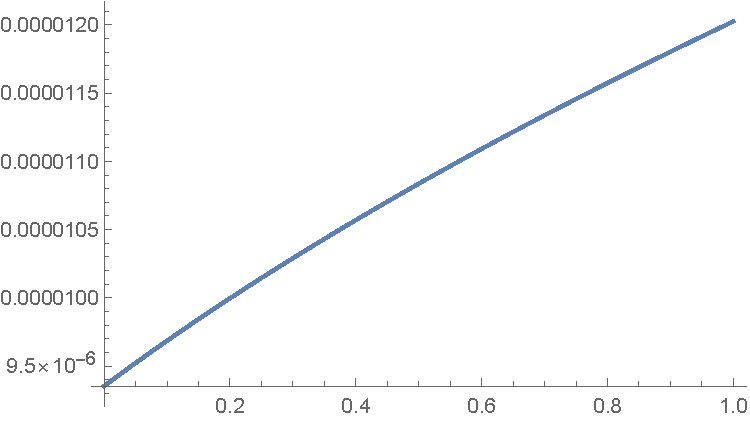
\includegraphics[width=1\textwidth]{Figures/Plot_dmdt_as_f_of_p.pdf}
  \caption{$\dbyd{M}{\tau}$ at EE as a function of $p$.}
\end{figure}
From the graph, we can claim that mortality per unit time is higher if $p$ is higher. Since $I$ approaches 0 at EE, there is almost no disease induced mortality from individuals that are not variolated. It is evident that in the long run, a higher rate of intentional infection will lead to more disease induced death.

\end{document}